% Capítulo 1: o ciclo requisição/resposta entre cliente e servidor.
\documentclass[border=4pt]{standalone}
\usepackage[utf8]{inputenc}
\usepackage[T1]{fontenc}
% Estilo comum dos fluxogramas e diagramas de blocos.
\usepackage{tikz}
\usetikzlibrary{arrows.meta, positioning, calc, shapes.geometric, shapes.misc}
\definecolor{navy}{RGB}{23,45,80}
\definecolor{laranja}{RGB}{250,110,29}
\definecolor{cinzalogo}{RGB}{107,114,126}
\definecolor{azul}{RGB}{205,222,247}
\tikzset{
  base/.style={draw=navy, line width=0.9pt, font=\sffamily\small, align=center, inner sep=4pt},
  terminal/.style={base, rounded rectangle, fill=laranja!45, draw=laranja, minimum width=20mm, minimum height=7mm},
  processo/.style={base, rectangle, fill=laranja!12, minimum width=28mm, minimum height=8mm},
  decisao/.style={base, diamond, aspect=2.2, fill=azul, inner sep=1pt, minimum width=30mm},
  es/.style={base, trapezium, trapezium left angle=72, trapezium right angle=108,
             fill=white, minimum width=26mm, minimum height=8mm, trapezium stretches body},
  fluxo/.style={-{Stealth[length=2.2mm]}, navy, line width=0.9pt},
  rotulo/.style={font=\sffamily\small\bfseries, text=navy},
  legenda/.style={font=\sffamily\scriptsize, text=cinzalogo},
  resposta/.style={font=\sffamily\scriptsize\bfseries, text=navy},
}

\tikzset{
  caixa/.style={base, rectangle, rounded corners=3pt, fill=laranja!12, minimum width=30mm, minimum height=22mm},
  msg/.style={base, rectangle, fill=white, font=\ttfamily\scriptsize, align=left, text width=50mm},
  nota/.style={font=\sffamily\scriptsize, text=cinzalogo, align=center},
}
\begin{document}
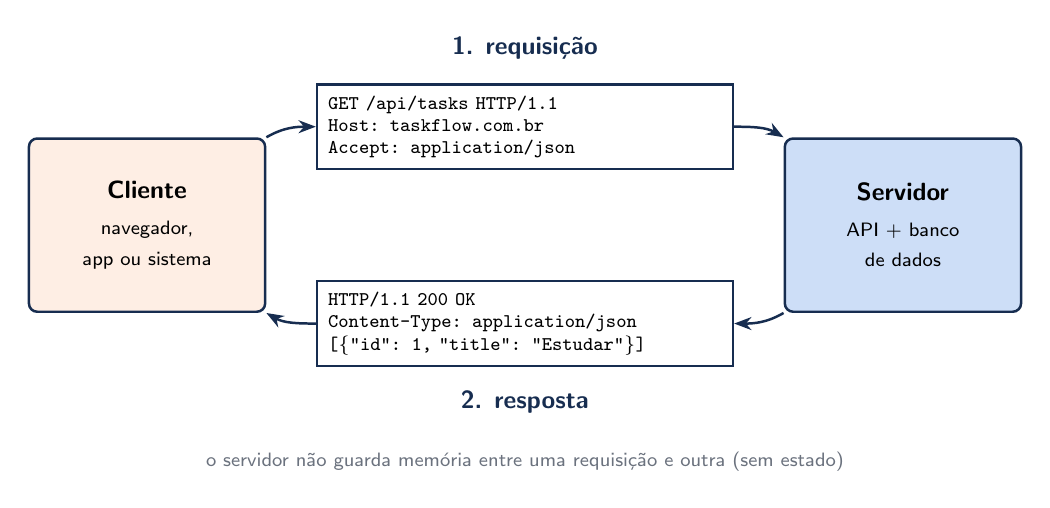
\begin{tikzpicture}
  \node[caixa] (cli) at (0, 0) {\textbf{Cliente}\\[2pt]\scriptsize navegador,\\\scriptsize app ou sistema};
  \node[caixa, fill=azul] (srv) at (9.6, 0) {\textbf{Servidor}\\[2pt]\scriptsize API + banco\\\scriptsize de dados};

  \node[msg] (req) at (4.8, 1.25) {GET /api/tasks HTTP/1.1\\Host: taskflow.com.br\\Accept: application/json};
  \node[msg] (res) at (4.8, -1.25) {HTTP/1.1 200 OK\\Content-Type: application/json\\{} [\{"id": 1, "title": "Estudar"\}]};

  \draw[fluxo] (cli.north east) to[out=30, in=180] (req.west);
  \draw[fluxo] (req.east) to[out=0, in=150] (srv.north west);
  \draw[fluxo] (srv.south west) to[out=210, in=0] (res.east);
  \draw[fluxo] (res.west) to[out=180, in=-30] (cli.south east);

  \node[rotulo] at (4.8, 2.25) {1. requisição};
  \node[rotulo] at (4.8, -2.25) {2. resposta};
  \node[nota] at (4.8, -3.0) {o servidor não guarda memória entre uma requisição e outra (sem estado)};
\end{tikzpicture}
\end{document}
